\documentclass[11pt]{article}

% -------------------- Packages --------------------
\usepackage[margin=1in]{geometry}
\usepackage{array}
\usepackage{longtable}
\usepackage{graphicx}
\usepackage{enumitem}
\usepackage{caption}
\usepackage{titlesec}
\usepackage{float}   % REQUIRED for [H] tables

% -------------------- Formatting --------------------
\setlist[itemize]{noitemsep, topsep=0pt}
\setlength{\parskip}{0.5em}
\setlength{\parindent}{0pt}

\captionsetup{
  justification=centering,
  labelfont=bf,
  textfont=normalfont
}

% -------------------- Document --------------------
\begin{document}

\begin{center}
\textbf{\Large Sri Sivasubramaniya Nadar College of Engineering, Chennai}\\
\textbf{(An Autonomous Institution affiliated to Anna University)}
\end{center}

\begin{table}[h]
\renewcommand{\arraystretch}{1.4}
\resizebox{\textwidth}{!}{%
\begin{tabular}{|l|l|l|l|}
\hline
Degree \& Branch & B.E. Computer Science \& Engineering & Semester & VI \\ \hline
Subject Code \& Name & \multicolumn{3}{l|}{UCS2612 – Machine Learning Algorithms Laboratory} \\ \hline
Academic Year & 2025–2026 (Even) & Batch & 2023–2027 \\ \hline
Name & Monesh M & Register No. & 3122235001084 \\ \hline
Due Date & \multicolumn{3}{l|}{06.01.2026} \\ \hline
\end{tabular}}
\end{table}

\begin{center}
\textbf{ Experiment 2:}
\textbf{Binary Classification using Naïve Bayes and K-Nearest Neighbors}
\end{center}

% --------------------------------------------------

\section*{1. Aim and Objective}
To implement Naïve Bayes and K-Nearest Neighbors (KNN) classifiers for a binary classification problem, evaluate them using multiple performance metrics, visualize model behavior, and analyze overfitting, underfitting, and bias–variance characteristics.

% --------------------------------------------------

\section*{2. Dataset Description}
The Spambase dataset is a benchmark binary classification dataset used to identify spam emails. It consists of numerical features extracted from email content and a binary class label indicating spam or non-spam.

\textbf{Dataset Reference:}
\begin{itemize}
\item Kaggle – Spambase Dataset
\end{itemize}

% --------------------------------------------------

\section*{3. Preprocessing Steps}
\begin{itemize}
\item Loaded the dataset using Pandas
\item Separated features and target labels
\item Performed stratified train–test split
\item Applied feature scaling using StandardScaler
\end{itemize}

% --------------------------------------------------

\section*{4. Implementation Details}
\begin{itemize}
\item Implemented Gaussian, Multinomial, and Bernoulli Naïve Bayes classifiers
\item Implemented baseline KNN classifier
\item Tuned KNN hyperparameters using GridSearchCV and RandomizedSearchCV
\item Compared KDTree and BallTree neighbor search algorithms
\end{itemize}

% --------------------------------------------------

\section*{5. Visualizations}

\begin{figure}[H]
\centering
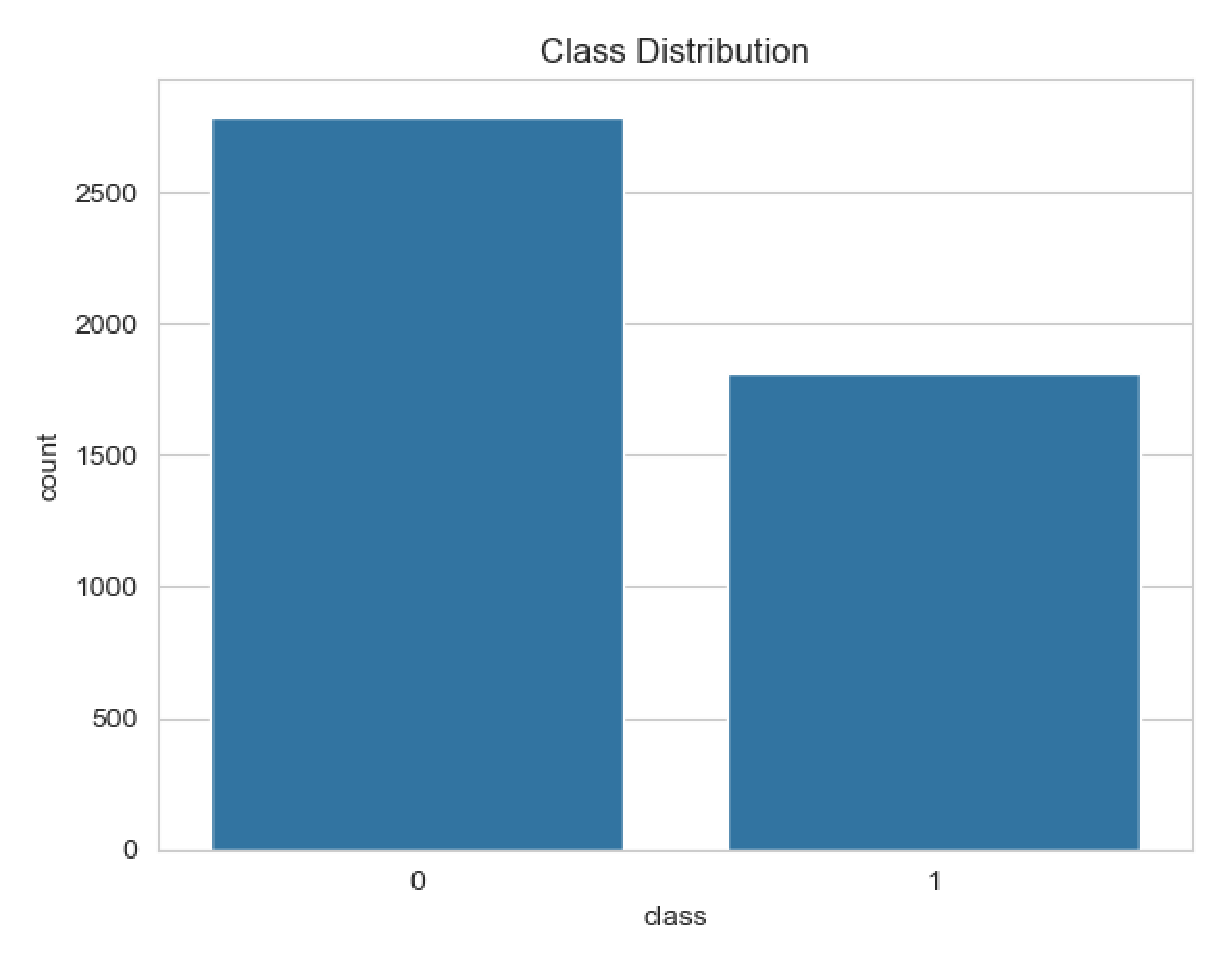
\includegraphics[width=0.65\textwidth]{image_eps/class_distribution.eps}
\caption{Class Distribution of Spam and Non-Spam Emails}
\end{figure}

\begin{figure}[H]
\centering
\includegraphics[width=0.85\textwidth]{image_eps/feature_distribution.eps}
\caption{Feature Distribution Plot (Sample Features)}
\end{figure}

\begin{figure}[H]
\centering
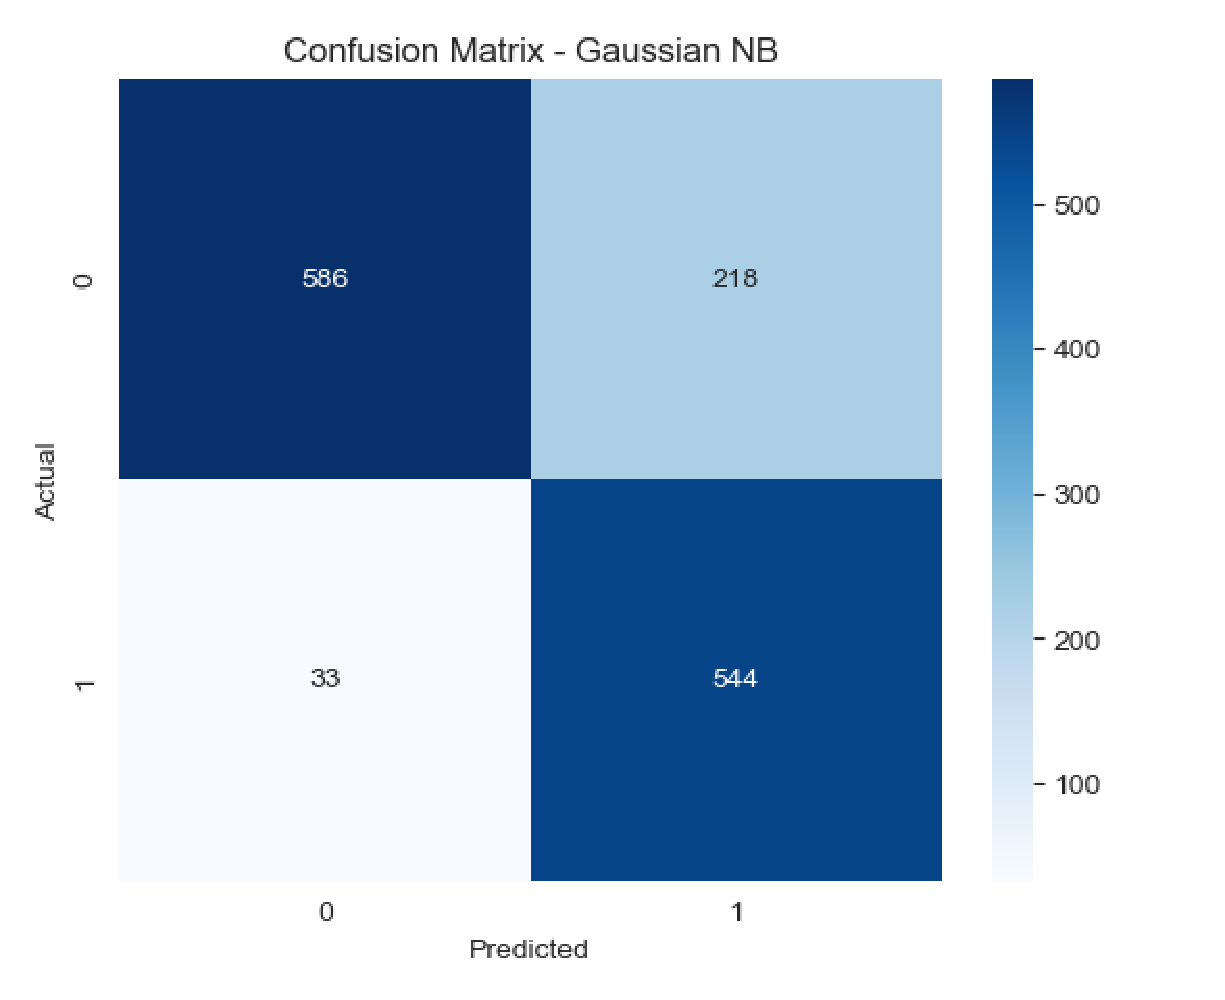
\includegraphics[width=0.55\textwidth]{image_eps/cm_GaussianNB.eps}
\caption{Confusion Matrix for Gaussian Naïve Bayes}
\end{figure}

\begin{figure}[H]
\centering
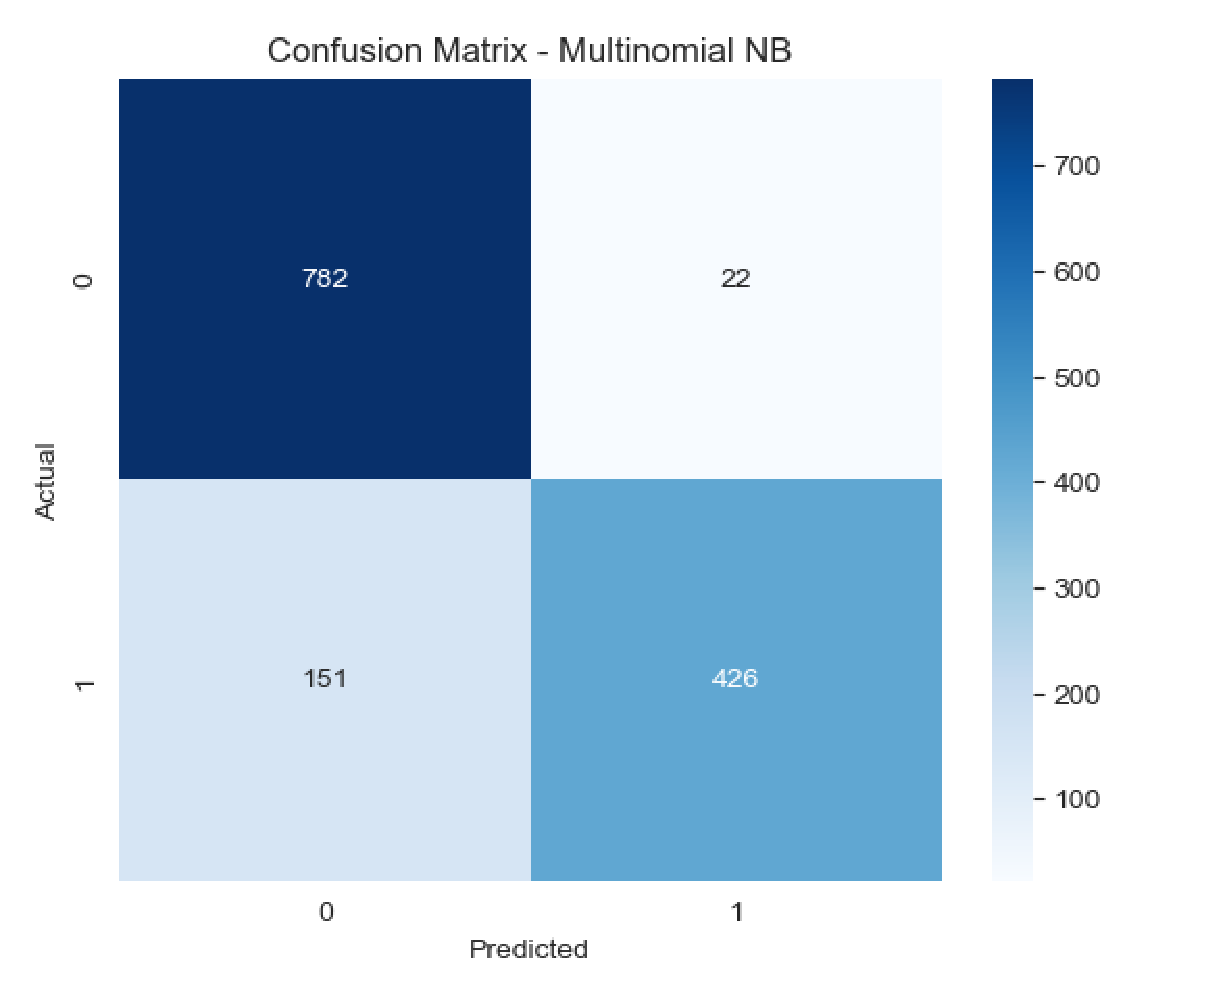
\includegraphics[width=0.55\textwidth]{image_eps/cm_MultinomialNB.eps}
\caption{Confusion Matrix for Multinomial Naïve Bayes}
\end{figure}

\begin{figure}[H]
\centering
\includegraphics[width=0.55\textwidth]{image_eps/cm_BernoulliNB.eps}
\caption{Confusion Matrix for Bernoulli Naïve Bayes}
\end{figure}

\begin{figure}[H]
\centering
\includegraphics[width=0.65\textwidth]{image_eps/roc_GaussianNB.eps}
\caption{ROC Curve for Gaussian Naïve Bayes}
\end{figure}

\begin{figure}[H]
\centering
\includegraphics[width=0.65\textwidth]{image_eps/roc_MultinomialNB.eps}
\caption{ROC Curve for Multinomial Naïve Bayes}
\end{figure}

\begin{figure}[H]
\centering
\includegraphics[width=0.65\textwidth]{image_eps/roc_BernoulliNB.eps}
\caption{ROC Curve for Bernoulli Naïve Bayes}
\end{figure}

\begin{figure}[H]
\centering
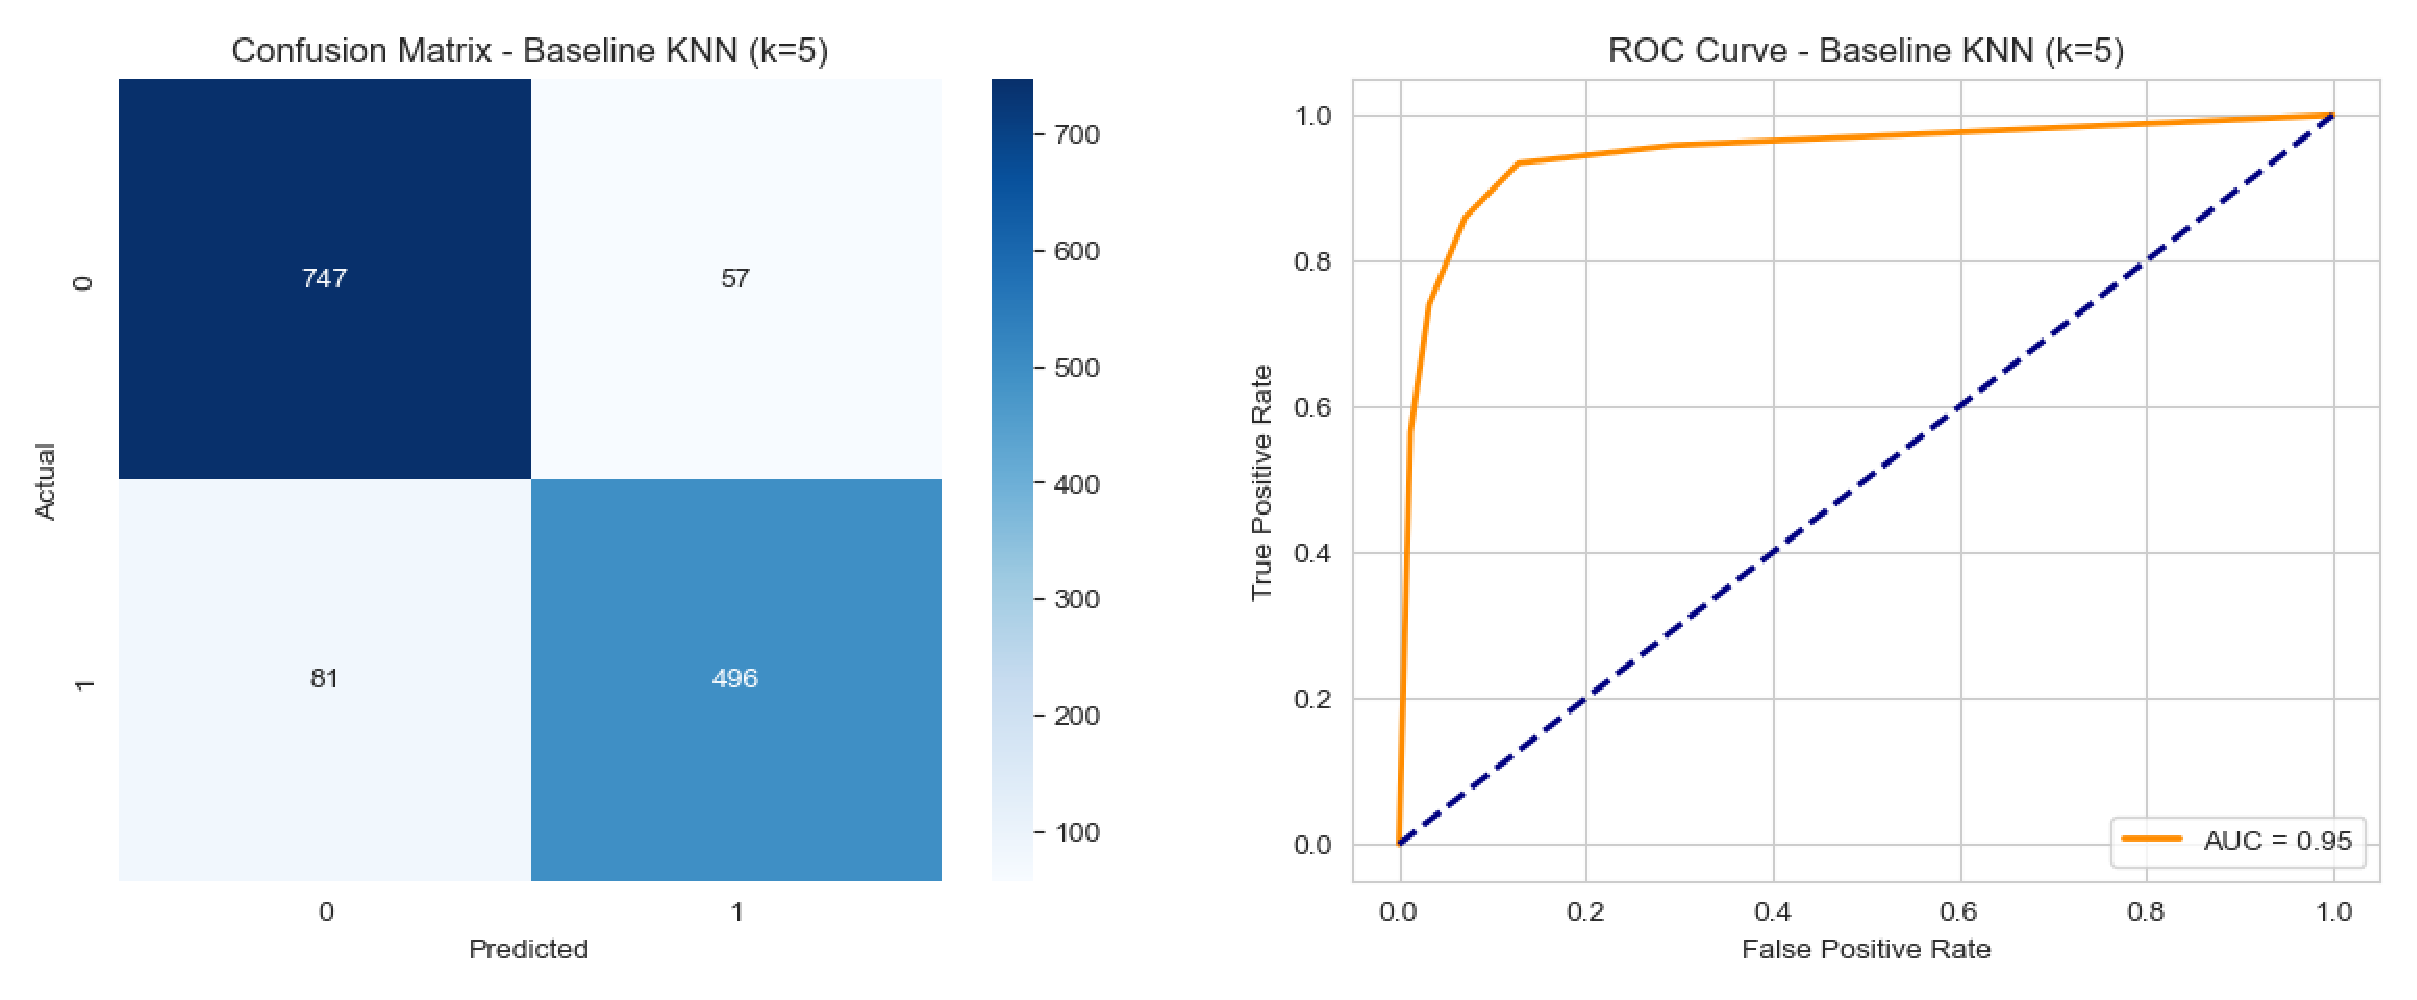
\includegraphics[width=0.7\textwidth]{image_eps/accuracy_vs_k.eps}
\caption{Accuracy vs. k Plot for KNN}
\end{figure}

\begin{figure}[H]
\centering
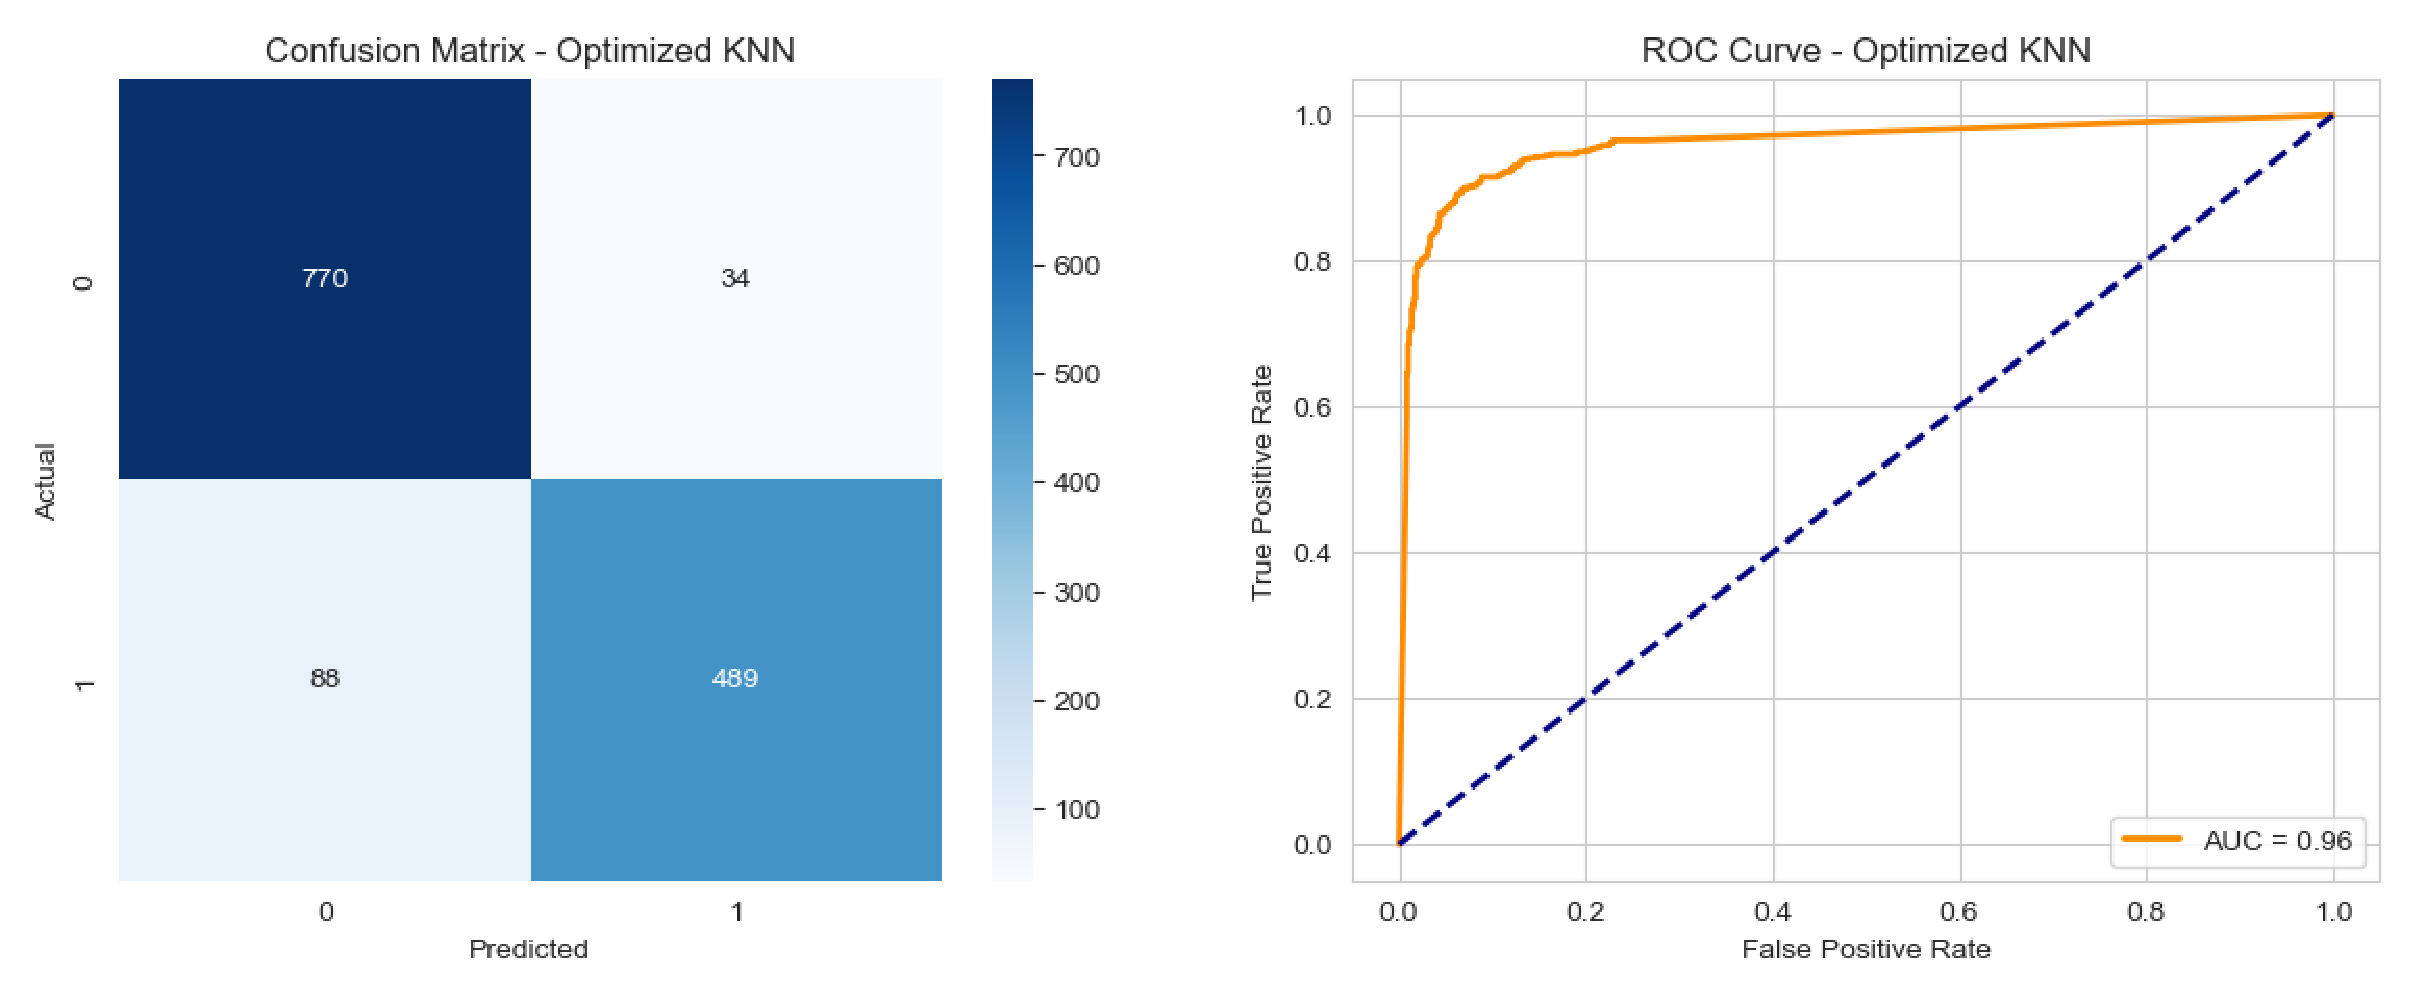
\includegraphics[width=0.7\textwidth]{image_eps/train_vs_validation.eps}
\caption{Training vs Validation Accuracy for KNN}
\end{figure}


% --------------------------------------------------

\section*{6. Performance Tables}

\begin{table}[H]
\centering
\caption{Naïve Bayes Performance Metrics}
\begin{tabular}{|l|c|c|c|}
\hline
\textbf{Metric} & \textbf{Gaussian NB} & \textbf{Multinomial NB} & \textbf{Bernoulli NB} \\ \hline
Accuracy & 0.8339 & 0.7763 & 0.8762 \\ \hline
Precision & 0.7178 & 0.7199 & 0.8716 \\ \hline
Recall & 0.9532 & 0.7080 & 0.8044 \\ \hline
F1 Score & 0.8189 & 0.7139 & 0.8367 \\ \hline
Specificity & 0.5495 & 0.6406 & 0.6382 \\ \hline
Training Time (s) & 0.0042 & 0.0027 & 0.0045 \\ \hline
\end{tabular}
\end{table}

\begin{table}[H]
\centering
\caption{KNN Hyperparameter Tuning}
\begin{tabular}{|l|c|c|}
\hline
\textbf{Search Method} & \textbf{Best Parameters} & \textbf{Best CV Accuracy} \\ \hline
Grid Search & k=15, distance, KDTree & 0.9209 \\ \hline
Randomized Search & k=15, distance, BallTree & 0.9209 \\ \hline
\end{tabular}
\end{table}

\begin{table}[H]
\centering
\caption{KNN Performance using KDTree}
\begin{tabular}{|l|c|}
\hline
\textbf{Metric} & \textbf{Value} \\ \hline
Optimal k & 15 \\ \hline
Accuracy & 0.9175 \\ \hline
Precision & 0.9065 \\ \hline
Recall & 0.8815 \\ \hline
F1 Score & 0.8939 \\ \hline
Training Time (s) & 0.0256 \\ \hline
Prediction Time (s) & 0.2356 \\ \hline
\end{tabular}
\end{table}

\begin{table}[H]
\centering
\caption{KNN Performance using BallTree}
\begin{tabular}{|l|c|}
\hline
\textbf{Metric} & \textbf{Value} \\ \hline
Optimal k & 15 \\ \hline
Accuracy & 0.9175 \\ \hline
Precision & 0.9065 \\ \hline
Recall & 0.8815 \\ \hline
F1 Score & 0.8939 \\ \hline
Training Time (s) & 0.0075 \\ \hline
Prediction Time (s) & 0.1619 \\ \hline
\end{tabular}
\end{table}

\begin{table}[H]
\centering
\caption{Comparison of Neighbor Search Algorithms}
\begin{tabular}{|l|c|c|}
\hline
\textbf{Criterion} & \textbf{KDTree} & \textbf{BallTree} \\ \hline
Accuracy & 0.9175 & 0.9175 \\ \hline
Training Time (s) & 0.0256 & 0.0075 \\ \hline
Prediction Time (s) & 0.2356 & 0.1619 \\ \hline
Memory Usage & Low / Medium & Medium / High \\ \hline
\end{tabular}
\end{table}

% --------------------------------------------------

\section*{7. Overfitting and Underfitting Analysis}
\begin{itemize}
\item Small values of k resulted in overfitting
\item Large values of k caused underfitting
\item Hyperparameter tuning improved generalization
\end{itemize}

% --------------------------------------------------

\section*{8. Bias–Variance Analysis}
\begin{itemize}
\item Naïve Bayes shows higher bias due to feature independence assumption
\item KNN exhibits higher variance for small k values
\item Hyperparameter tuning balances bias–variance trade-off
\end{itemize}

% --------------------------------------------------

\section*{9. Observations and Conclusion}
Naïve Bayes classifiers were computationally efficient, while tuned KNN models achieved higher accuracy. BallTree demonstrated better computational efficiency compared to KDTree. Proper preprocessing, visualization, and hyperparameter tuning significantly improved model performance and generalization.

\section*{References}
\begin{itemize}
\item Scikit-learn – Naïve Bayes Documentation
\item Scikit-learn – KNN Documentation
\item Scikit-learn – Hyperparameter Optimization
\item Kaggle – Spambase Dataset
\end{itemize}

\end{document}
